En 1565, el médico y botanista Nicolás Monardes reportó el peculiar color azul que tomaba una infusión de madera mexicana usada para tratar enfermedades de riñón y urinarias. Este efecto ya era conocido por los Aztecas, que lo utilizaban para asegurarse que la valiosa madera no fuera falsificada. Monardes escribe en su libro \cite{valeur_introduction_2012}

\begin{quote}
    \textit{Asegúrate de que la madera torne el agua azulada, de lo contrario, es una falsificación. De hecho, ahora traen otro tipo de madera que torna el agua amarilla, pero no sirve; solo el tipo que torna el agua azulada es genuina.}
\end{quote}  

\noindent Años más tarde, en 1845, el matemático Sir John Herschel describió el efecto similar que producía una solución transparente de quinina, una sustancia presente en el agua tónica, que reflejaba \flqq un color azul celestial hermoso y extremadamente vívido\frqq.
Herschel usó un prisma para comprobar que la dispersión causada por la quinina sólo se observaba al iluminar la solución con la parte azul del espectro.
El mismo análisis para la luz emitida reveló luz azul, verde, y una pequeña cantidad de amarillo.
En esa misma época, el físico Sir George Gabriel Stokes publicó \textit{On the Refrangibility of Light}, un trabajo explicando experimentos con múltiples sustancias que exhibían este tipo de comportamientos, entre ellas incluida la quinina.
Uno de sus experimentos más importantes consistía en formar el espectro solar a partir de un prisma, para luego mover un tubo de ensayo con la solución de quinina a través de sus colores.
La solución permanecía transparente al ser iluminada por la parte visible del espectro, pero al llegar a la zona ultravioleta (invisible al ojo humano), la muestra se iluminó con luz azul brillante.
Además de concluir que la luz siempre se dispersaba con longitudes de onda mayores a las de incidencia, afirmación que luego se conocería como corrimiento de Stokes, llamó a este fenómeno \textit{fluorescencia} \cite{valeur_introduction_2012}.

En 1888, el físico Eilhardt Wiedmann introdujo el término luminiscencia para referirse a los fenómenos lumínicos que no están determinados por un aumento en la temperatura de los materiales.
Entre ellos están la fosforescencia y la fluorescencia.
Actualmente ambos tienen aplicaciones en múltiples áreas distintas del conocimiento y la tecnología. 
Es particularmente destacable su éxito como herramienta para estudiar la estructura y dinámica de la materia viva, gracias la sensibilidad al micro-entorno de las moléculas fluorescentes, lo que resulta en una alta resolución espacial y temporal. 
Por ejemplo, la microscopía de fluorescencia consiste en iluminar la muestra con una longitud de onda y detectar su fluorescencia en otra, permitiendo filtrar el fondo de la imagen \cite{valeur_introduction_2012}.
Técnicas dinámicas como la microscopía de imágenes de tiempo de vida de fluorescencia (FLIM) o fosforescencia (PLIM) dan lugar a conocer el entorno químico en el que se encuentran distintas proteinas, como su PH, viscosidad, temperatura, entre otras cantidades \cite{suhling_fluorescence_2015} \cite{baggaley_timeresolved_2015}.
Si bien en el siglo 19 ya se sabía que los mecanismos de emisión de luz de estos fenómenos no estaban vinculados al aumento de temperatura de los materiales, no fue hasta el desarrollo de la mecánica cuántica a principos del 20 que se entendió su causa: la luminiscencia está dada por la transición entre distintos estados de energía de los electrones.

\section{Luminiscencia}


\begin{figure}
    \centering
    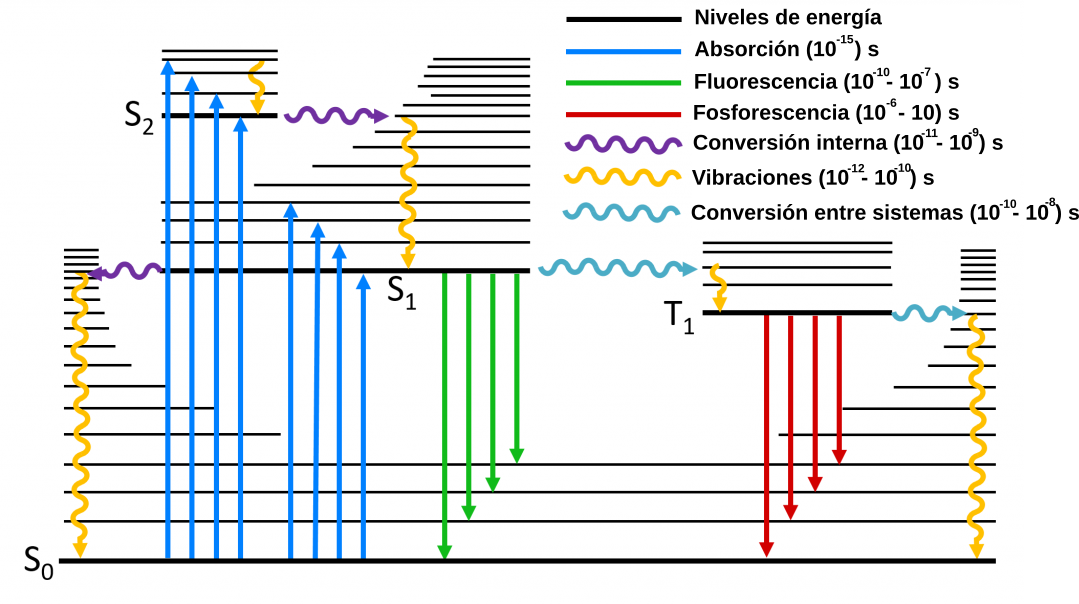
\includegraphics[width=\textwidth]{jablonski}
    \caption{\textbf{Diagrama de Jablonski.} En negro se ven los niveles de energía, crecientes en el eje vertical. Las flechas de colores muestran las transiciones posibles. Tomado de $^1$.}
    \label{fig:jablonski}
\end{figure}

\subsection{Espectroscopía estacionaria}

La luminiscencia es la emisión de fotones mediante la transición de un electron en un estado excitado con energía $E_e$ a otro con energía $E_k < E_e$.
Este proceso suele ilustrarse a través de un diagrama de Jablonski (\textbf{Fig. \ref{fig:jablonski}})\footnote{Tomado de \href{https://edinst.com/wp-content/uploads/2019/02/JablonskiDiagramFull-1024x604.png}{https://edinst.com/wp-content/uploads/2019/02/JablonskiDiagramFull-1024x604.png}}.
En un diagama de Jablonski se muestran los niveles de energía electrónicos del material luminiscente junto con las posibles transiciones entre ellos.
En el diagrama se ven los estados singlete $S_0$, $S_1$ y $S_2$, y el estado triplete $T_1$.
Todo proceso luminiscente comienza con la absorción de un fotón, lo que lleva al electrón a un estado más energético.
Estas absorciones ocurren en un lapso de $10^{-15}$ s, un tiempo suficientemente corto como para que los desplazamientos de los núcleos del sistema sean despreciables \cite{lakowicz_principles_2006}.
La diferencia de energía entre estos estados es típicamente del orden de los eV.
A su vez, un electrón en un dado estado electrónico puede estar en distintos estados vibracionales, aunque estos estados están separados por energías del orden de las décimas de eV.
Las transiciones entre estados vibracionales también son posibles y ocurren en un lapso de $10^{-12}$ a $10^{-10}$ segundos.

La sucesión de este tipo de transiciones da lugar a la fluorescencia: un electrón absobe un fotón altamente energético, excitándolo a un estado electrónico de mayor energía con vibraciones.
Rápidamente sus oscilaciones se relajan, dejándolo en un estado electrónico excitado, pero con baja energía vibracional.
Por último, el electrón vuelve a su estado fundamental re-emitiendo un fotón, pero esta vez de menor energía que el que había absorbido.
La fluorescencia tiene tiempos típicos de $10^{-10}$ a $10^{-7}$ segundos.
El método más usual para caracterizar un material fluorescente, o luminiscente en general, es a través de su espectro de emisión y de absorción.
Alternativamente, uno puede medir el espectro de excitación, que está fuertemente relacionado con el de absorción.
El proceso para medir cada uno es:

\begin{itemize}
    \item \textbf{Emisión:} consiste en medir la intensidad de luz emitida por la muestra en un rango amplio de longitudes de onda $\Delta \lambda_{em}$, al ser excitada por una longitud de onda fija $\lambda_{ex}$.
    \item \textbf{Absorción:} requiere medir la intensidad de luz que absorbe la muestra. Esto generalmente se logra excitando una solución de la sustancia en un rango de longitudes de onda y midiendo la cantidad de luz transmitida en cada caso.
    \item \textbf{Excitación:} para obtener este espectro se debe medir la intensidad de luz emitida por la muestra una dada longitud de onda $\lambda_{em}$, y barrer la excitación en un rango $\Delta \lambda_{ex}$.
\end{itemize}

\noindent La figura (\textbf{\ref{fig:fluoresceina}}) muestra el espectro de absorción y de emisión de la fluoresceina, una tinta orgánica utilizada en distintas técnicas de diagnóstico médico \cite{fluoresceina_1,fluoresceina_2}.
Los espectros dejan en evidencia la fluorescencia de la molécula: absorbe fotones de $457$ y $486$ nm, es decir $2.71$ eV y $2.55$ eV respectivamente, y emite con mayor intensidad en $523$ nm, equivalente a $2.37$ eV.
Previsiblemente, la diferencia de energía es de $\sim 0.2$ eV, en el rango de energías vibracionales.


\begin{SCfigure}
    \centering
    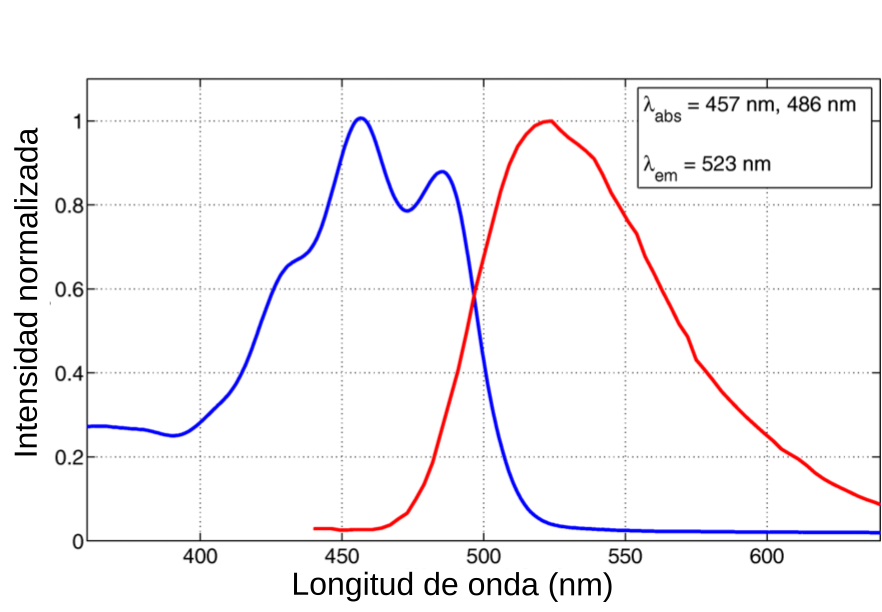
\includegraphics[width=0.7\textwidth]{fluoresceina_espectro.png}
    \caption{\textbf{Espectro de la Fluoresceina} diluida en etanol, tanto de absorción (azul) como de emisión (rojo). El cuadro muestra los picos de absorción en $\lambda_{abs}=457$ nm y 486 nm, y de emisión en $\lambda_{em}$ = 523 nm. Tomada y adaptada de \cite{kristoffersen_testing_2018}.}
    \label{fig:fluoresceina}
\end{SCfigure}

Otro tipo de mecanismos presentes en las moléculas luminiscentes son la conversión interna y la conversión entre sistemas.
Ambos consisten en transiciones entre estados electrónicos excitados, el primero es entre estados de la misma multiplicidad, en general singlete-singlete, y el segundo se da entre estados singlete-triplete \cite{valeur_characteristics_2012}.
La conversión entre sistemas, que ocurre en el orden de $10^{-10}$ a $10^{-9}$ segundos, es la responsable de la fosforescencia.
La fosforescencia es la transición de un electrón en un estado excitado triplete a un estado singlete de menor energía.
A diferencia de las transiciones fluorescentes, las transiciones triplete-singlete están prohibidas por las reglas de selección de la mecánica cuántica \cite{demtroder_emission_2010}.
Por este motivo, los tiempos característicos de la fosforescencia son mucho mayores, del orden de $10^{-6}$ hasta $10$ segundos.
Además de los espectros de absorción, emisión y excitación, los tiempos de estas transiciones son de gran relevancia para caracterizar a los materiales luminiscentes.

\subsection{Espectroscopía dinámica} \label{sec:dinamica}



Se le llama tiempo de vida medio al tiempo promedio que el electrón pasa en un estado excitado de energía.
La caracterización del tiempo de vida medio no solo brinda información del elemento luminiscente, sino también de su entorno.
Es necesario hablar de tiempos medios porque las transiciones son un fenómeno fundamentalmente cuántico, y por lo tanto un proceso aleatorio.
Además, la mayoría de mediciones de luminiscencia se hacen con una muestra que presenta grandes cantidades de los elementos ópticamente activos, por lo que también hay un efecto aleatorio propio de esa estadística.

\begin{SCfigure}
    \centering
    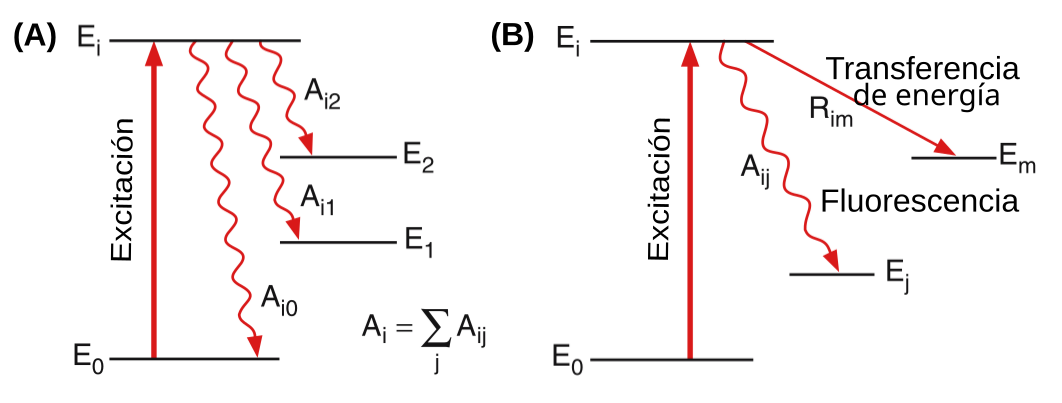
\includegraphics[width=0.7\textwidth]{transiciones_tiempo.png}
    \caption{\textbf{Diagrama de Jablonski} con transiciones que contribuyen al tiempo de vida.\textbf{(A)} Sólo transiciones de fluorescencia. \textbf{(B)} Transiciones de fluorescencia y transferencia de energía. Tomado y adaptado de \cite{demtroder_emission_2010}.}
    \label{fig:transiciones_tiempo}
\end{SCfigure}

Si se tienen $N_i$ átomos en un estado excitado con energía $E_i$ y se asume que la probabilidad de transición a un estado de menor energía $E_j$ es constante en el tiempo se obtiene que

\begin{equation} \label{eq:lifetime}
    \frac{dN_i}{dt} = \sum_j A_{ij} N_i \implies N_i(t) = N_i(0)e^{A_i t},
\end{equation}

\noindent donde $A_{ij}$ es una constante llamada coeficiente de Einstein, y $A_i = \sum_{j} A_{ij}$ tiene en cuenta la probabilidad del electrón decaiga a cualquier estado con $E_j < E_i$ (ver \textbf{Fig. \ref{fig:transiciones_tiempo}A}) \cite{demtroder_emission_2010}.
Como sabemos que un electrón emite un fotón al desexcitarse, la ecuación (\ref{eq:lifetime}) nos dice que al dejar de iluminar una muestra esperamos que se emitan fotones exponencialmente distribuidos en el tiempo.
Además sabemos que la relación entre el tiempo de vida y el parámetro de la exponencial es $\tau_i = 1/A_i$, por lo que es posible ajustar los datos para medirlo.
Exactamente eso es lo que se hace en \textit{Time-Correlated Single Photon Counting} (TCSPC, ver sección \ref{sec:intro_tcspc}), una de las técnicas más comunes para medir tiempos de vida.

La ecuación (\ref{eq:lifetime}) sólo tiene en cuenta las transiciones fluorescentes del átomo, pero como explicamos en la sección anterior, éstas no son las únicas.
Además, generalmente los átomos están en entornos que inducen transiciones no radiativas, como transferencia de energía a otros átomos, o colisiones con átomos vecinos (\textbf{Fig. \ref{fig:transiciones_tiempo}B}). 
Suponiendo que se induce una nueva probabilidad de desexcitación no radiativa $R_i$ por transferencia de energía, y siguiendo la lógica anterior, la tasa de cambio de cantidad de átomos $N_i$ en el estado $i$ es

\begin{equation} \label{eq:lifetime_choques}
    \frac{dN_i}{dt} = (A_{ij} + R_i) N_i \implies N_i(t) = N_i(0)e^{(A_i + R_i) t},
\end{equation}

\noindent y por lo tanto su tiempo de vida efectivo $\tau_{eff} = 1/(A_i + R_i)$. 
La implicancia de este fenómeno es muy fuerte: es posible obtener información del entorno microscópico de un material luminiscente al medir su tiempo de vida \cite{ryder_timedomain_2001}.

Para poder aprovechar estas propiedades de los materiales luminiscentes es necesario poder medir precisamente tanto sus espectros estacionarios como los dinámicos. 
En la próxima sección comentamos brevemente cuáles son los instrumentos y técnicas que se implementan más comunmente para hacer este tipo de mediciones.


\section{Instrumentación para espectrometría de fluorescencia}

\subsection{El espectrofluorímetro}

Para caracterizar la respuesta óptica de una sustancia, generalmente se desea registrar tanto el espectro de excitación como el de emisión. 
El instrumento científico por excelencia para realizar estas mediciones es el espectrofluorímetro. 
Fundamentalmente, este instrumento permite realizar mediciones de la intensidad de luz que emite una muestra, haciendo barridos en longitud de onda de emisión y excitación.
Adicionalmente, algunos pueden realizar mediciones de tiempo de vida resueltas, escaneos sincrónicos con alguna señal y mediciones de anisotropía en la polarización de materiales luminiscentes.
Estas capacidades son fundamentales para investigaciones en diversas disciplinas científicas, incluyendo química, bioquímica, farmacología, ciencias ambientales, ciencia de materiales y biomedicina.
El objetivo principal de un espectrofluorímetro es obtener los espectros de emisión y de excitación de una muestra.
Para lograr este objetivo, el instrumento debe ser capaz de iluminar la muestra con múltiples longitudes de onda diferentes y registrar su respuesta a cada una de ellas.

La figura (\textbf{\ref{fig:spec_diagram_lako}}) muestra un diagrama esquemático de un espectrofluorímetro genérico.
Este instrumento incluye todos los componentes fundamentales para cumplir su función. 
Utiliza una lámpara de espectro amplio que funciona como fuente de luz de alta intensidad para un rango extenso de longitudes de onda. 
Posteriormente la luz es filtrada por un monocromador de excitación que permite seleccionar la longitud de onda con la que se desea iluminar a la muestra.
La luz de excitación seleccionada se enfoca sobre la muestra colocada en la cámara principal, cuya luminiscencia, generalmente con una longitud de onda mayor que la luz de excitación, es filtrada por el monocromador de emisión.
Los monocromadores suelen estar motorizados, lo que permite que el barrido sea automático. 
La luz restante llega a un detector, usualmente un tubo fotomultiplicador (PMT), un detector muy sensible que convierte fotones en corriente eléctrica.
El espectrofluorímetro emplea diversas técnicas para reducir la luz parásita (longitudes de onda diferentes a la deseada), como el diseño en ángulo de 90° entre los brazos de excitación y emisión, y un compartimento hermético pintado de negro no reflectante.
La señal del PMT es procesada electrónicamente, digitalizada y analizada en una computadora. 
Este sistema también controla los monocromadores y la adquisición de datos, además de permitir al usuario ajustar parámetros y facilitar la visualización y análisis.
A menudo, se incorporan componentes adicionales en el camino óptico, como obturadores, polarizadores, divisores de haz y otros elementos ópticos, para estudiar diferentes propiedades de la muestra.

\begin{SCfigure}
     \centering
     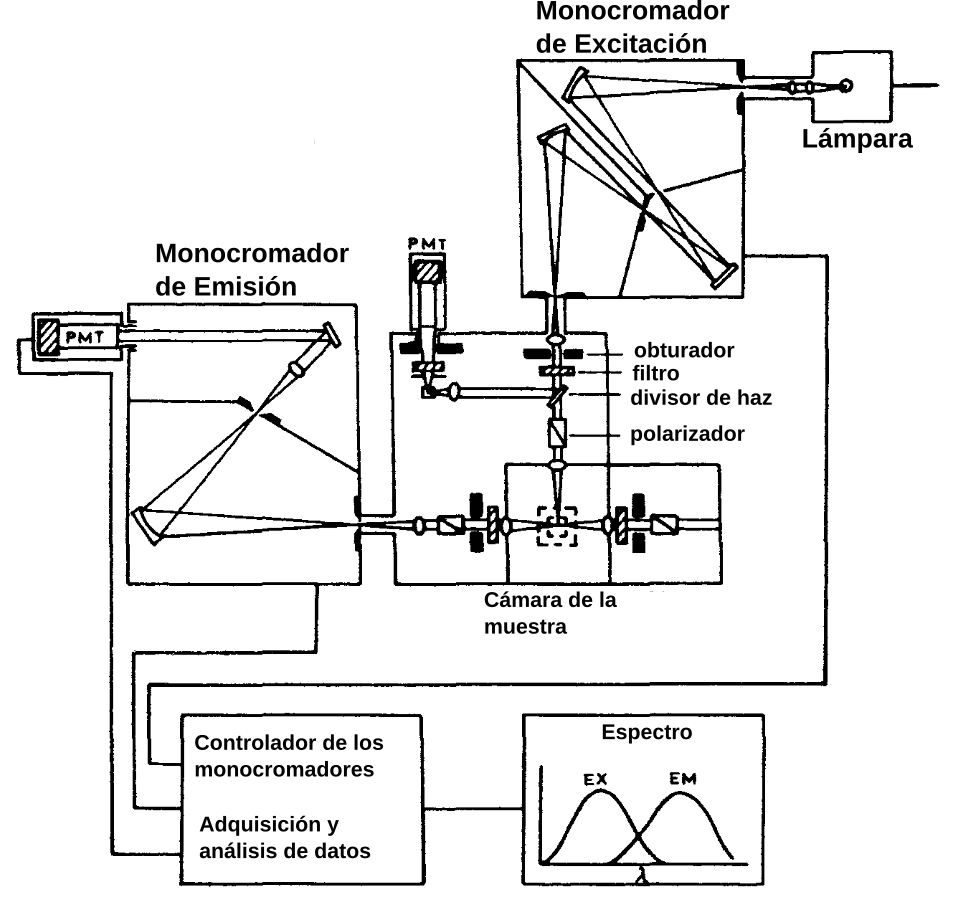
\includegraphics[width=0.6\textwidth]{spectrometer_diagram_lako_modif.png}
     \caption{
    \textbf{Diagrama de un espectrofluorímetro típico.}
    La luz traza un camino que comienza en la lámpara (zona superior derecha) y termina en el PMT de detección (centro-izquierda). Después de salir de la lámpara, la luz es filtrada por un monocromador y luego enfocada sobre la muestra. La luz reemitida pasa por otro monocromador y termina en el PMT. La señal se lee con un sistema de control que la digitaliza y para luego ser procesada por una PC que construye los espectros. Figura tomada y adaptada de \cite{lakowicz_principles_2006}.
    }
     \label{fig:spec_diagram_lako}
\end{SCfigure}


Actualmente, el Departamento de Física de la FCEyN-UBA no cuenta con espectrofluorímetros como el descripto en la sección anterior para la caracterización de espectros de excitación y emisión.  
En cambio, cuenta con espectrómetros CCD a fibra óptica como los CCS100 de THORLABS, los cuales no permiten seleccionar la longitud de onda de excitación, y tienen una relación señal-ruido 10 veces menor que la del QM 400. 
Para medir este tipo de espectros, la facultad dispone del laboratorio de fotoquímica del Instituto de Química Física de los Materiales, Medio Ambiente y Energía (INQUIMAE), que cuenta con tres espectrofluorímetros con distintas características, pero que tienen algo en común: ningún equipo tiene menos de 20 años, el más antigüo llegando a los 40 años de uso.
La disparidad en la antigüedad y funcionalidad de los instrumentos es un fenómeno común en laboratorios de investigación en países como Argentina, donde la inversión en ciencia es escasa o poco regular en el tiempo \cite{cioccaRealityScientificResearch2017}. 
Ante esta realidad, los institutos suelen priorizar la adquisición de equipos con nuevas capacidades, en lugar de renovar instrumentos existentes por versiones más modernas.  
Esto es posible gracias a la precisión y robustez de las partes mecánicas de los instrumentos, pero la obsolescencia de los equipos antiguos plantea problemas a largo plazo, especialmente cuando sus plataformas de control quedan desactualizadas.  
Con el tiempo, se vuelve complicado operar estos instrumentos, ya que los mecanismos de extracción de datos, como los disquetes, dejan de estar disponibles en el mercado. 
Aún más crítico es que el funcionamiento del equipo depende de la computadora de control, la cual utiliza placas y puertos que ya no se fabrican ni se consiguen en el mercado actual.  
El problema de la obsolescencia en instrumentos científicos afecta desproporcionadamente a instituciones con bajo presupuesto, ampliando la brecha de accesso a instrumentos de investigación avanzados.

Esto ha llevado a un auge en el desarrollo de instrumentos científicos accesibles y de bajo costo \cite{wenzel_open_2023, arancio_inequalities_2023}, particularmente en áreas como instrumentación, microscopía, espectroscopía y adquisición de datos \cite{jameson_fluorescent_1989, li_optical_2022, hu_fluorescent_2022}.
Las iniciativas de hardware abierto hacen que los diseños y la documentación estén disponibles de forma gratuita para que cualquier persona pueda usarlos, construirlos y modificarlos \cite{powell_democratizing_2012, oellermann_open_2022}.
Por ejemplo, la plataforma Arduino ha proporcionado una plataforma de desarrollo de electrónica económica y fácil de usar basada en un microcontrolador (https://www.arduino.cc/).
El OpenFlexure Microscope es un microscopio de código abierto que cuesta menos de 100 USD construir \cite{collins_robotic_2020}.
Asimismo, recientemente se desarrolló un espectrómetro basado en Raspberry Pi que cuesta menos de 400 EUR \cite{tunens_optical_2024}.
El software y los lenguajes de código abierto, como Python (http://www.python.org), que cuentan con bibliotecas numéricas y de instrumentación como NumPy \cite{harris_array_2020} y PyVISA \cite{grecco_pyvisa_2023}, han desempeñado un papel clave al reducir las barreras de entrada y facilitar la creación rápida de prototipos.
Cabe destacar que han surgido empresas enfocadas en hardware parcialmente o completamente abierto. Por ejemplo, OpenBCI (https://openbci.com/), que ofrece sistemas EEG de bajo costo para interfaces cerebro-computadora, y Opentrons (https://opentrons.com/), que proporciona soluciones de manejo de líquidos para la automatización de laboratorios.


\subsection{Medición de tiempos de vida: \textit{Time-Correlated Single Photon Counting}} \label{sec:intro_tcspc}


\begin{figure}
    \centering
    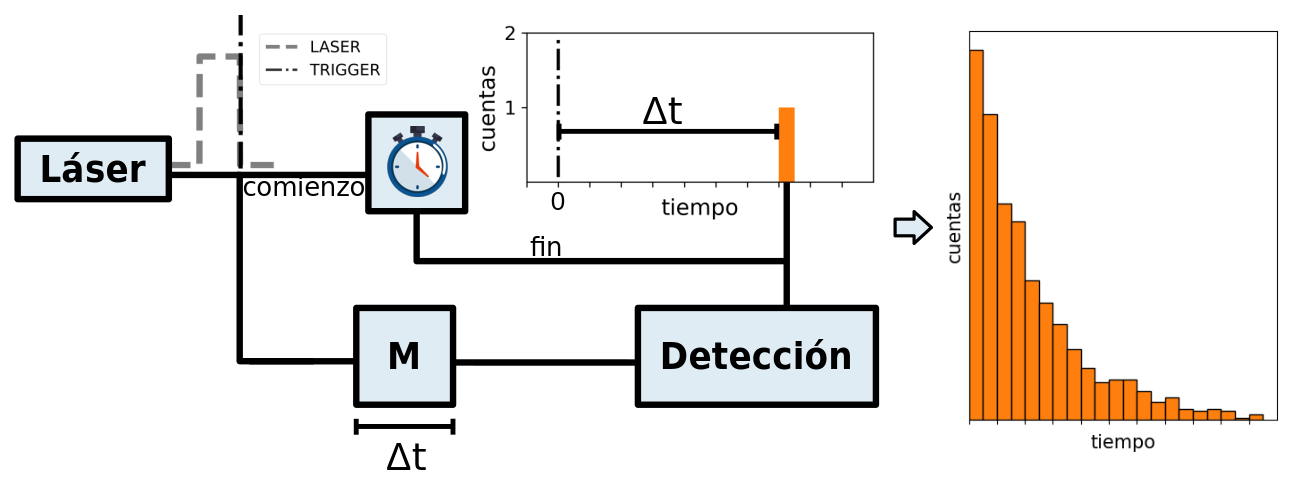
\includegraphics[width=\textwidth]{tcspc.png}
    \caption{\textbf{Diagrama de TCSPC.} El láser envía un pulso que excita a la muestra e inicia un cronómetro. La muestra tarda un tiempo $\Delta t$ en re-emitir. El sistema de detección detecta la luz y pone detiene el cronómetro. Se registra el tiempo $\Delta t$. Al repetir el experimento múltiples veces se crea el histograma de cuentas en función del tiempo (derecha). Adaptada de \cite{bujjamer2020}.}
    \label{fig:tcspc}
\end{figure}

Muchos espectrofluorímetros comerciales tienen la capacidad de medir tiempos de vida del orden de los nanosegundos. 
Sin embargo, existen materiales luminiscentes, como los fosforescentes, presentan tiempos de vida del orden de los cientos de microsegundos en adelante.
Aunque esto alivia la necesidad de una electrónica rápida y costosa, contradictoriamente hace que no se pueda medir su tiempo de vida en instrumentos comerciales, ya que los valores típicos están muy alejados del rango en el que operan \cite{bujjamer2020}.

Existen distintas técnicas para medir el tiempo de vida \cite{becker_fluorescence_2012}, pero la más implementada es \textit{Time-Correlated Single Photon Counting} (TCSPC).
TCSPC es una técnica digital que cuenta fotones correlacionados temporalmente con respecto a un pulso de excitación.
Un diagrama de esta técnica de medición se puede ver en la figura (\textbf{\ref{fig:tcspc}}).
El experimento comienza con un pulso de excitación, que tiene dos tareas: (i) excitar a la muestra y (ii) iniciar algún tipo de cronómetro.
La muestra se excita repetidamente utilizando una fuente de luz pulsada, comunmente un láser.
Cada pulso es monitoreado, produciendo una señal de inicio que activa el contador del cronómetro.
Usualmente, para esta tarea se usa un discriminador de fracción constante (CFD) para detectar el pulso, y un conversor de tiempo a amplitud (TAC) para medir el tiempo.
La luz re-emitida por la muestra llega al sistema de detección, que además de detectar el pulso es el responsable de detener el cronómetro.
Al final de esta medición se obtiene el tiempo que tardó el fotón en llegar al detector.
Al repetir este experimento múltiples veces, se construye un histograma de cuentas de fotones en función del tiempo.
De acuerdo a lo explicado en la sección \ref{sec:dinamica}, para el caso en que sólo hay transiciones de fluorescencia, las alturas de las barras de este histograma deberían seguir una distribución exponencial con tiempo característico $\tau$, el tiempo de vida.

Además de los sistemas fluorescentes y fosforescentes existen otros sistemas en los que distintos centros ópticamente activos interactúan entre sí de forma no lineal, resultando en que la solución a la ecuación equivalente a \ref{eq:lifetime_choques} no sea una exponencial decreciente.
En la próxima sección introduciremos a las nanopartículas de \textit{upconversion}, un sistema con estas propiedades.


\section{Nanopartículas de \textit{upconversion}} \label{sec:intro_ucnp}

\subsection{Luminiscencia de las UCNP}

Las nanopartículas de \textit{upconversion} (UCNP) consisten en una matriz cristalina con dimensiones nanométricas dopada con iones lantánidos trivalentes.
El término \textit{upconversion}, que traducido literalmente del inglés sería conversión ascendente, surge la capacidad de las UCNP de absorber fotones de baja energía, generalmente en el infrarrojo cercano (NIR) y re-emitirlos en el espectro visible y ultravioleta (UV-VIS).
Esta propiedad encuentra aplicaciones en distintas tecnologías.
Por ejemplo, se pueden utilizar como trazadores ópticos en microscopía para etiquetar células, manipular drogas a nivel microscópico y en teranósticos, una técnica de diagnóstico usada comunmente en tratamientos de medicina nuclear \cite{shen_lanthanidedoped_2013,guryev_ucnpbased_2020,haase_upconverting_2011}.
Al absorber en el infrarrojo presentan una ventaja ante otros fluoróforos, ya que en este rango de longitudes de onda la luz es menos dispersada por los tejidos, además de causar menos daño biológico.
Esta capacidad de convertir luz en el NIR al UV-VIS también se puede aprovechar para mejorar la eficiencia de celdas solares, que no son capaces de convertir fotones en el NIR a energía eléctrica \cite{hao_enhancing_2017}.
Otras potenciales aplicaciones de las nanopartículas incluyen su uso para el diseño de pantallas transparentes, termómetros nanométricos y detectores de moléculas fluorescentes en agua \cite{hong_orthogonal_2021,savchuk_thermochromic_2016, bujjamer_first_2021}.

El motivo de la conversión ascendente de las nanopartículas está dado por la interacción entre los iones lantánidos con las que son dopadas.
Los lantánidos son los elementos del sexto período de la tabla periódica, y se caracterizan por ser los elementos que completan los niveles electrónicos $4f$, comenzando con el lantano y finalizando con el lutecio.
Aunque esos son sus niveles más energéticos sin completar, los niveles $5s^25p^6$ corresponden a funciones de onda más externas que las $4f$, generando una especie de capa protectora para los electrones de valencia \cite{lanthanides}.
La consecuencia de esto son bandas muy angostas en sus espectros de emisión, ya que sus propiedades se ven poco afectadas por los factores externos. 
Por este motivo, los niveles de energía de los iones lantánidos dentro de la matriz cristalina son similares sus niveles cuando están libres\cite{nadort_lanthanide_2016}.
La luminiscencia de estos iones se da por las transiciones entre los niveles $f-f$ con la misma paridad.
Si bien las reglas de selección de la mecánica cuántica establecen que estas transiciones están prohibidas por dipolo eléctrico, para los lantánidos que se encuentran en las UCNP estas condiciones se ven relajadas por la asimetría de la red cristalina y la interacción entre ellos \cite{basics_of_lanthanide}.
Estas transiciones semi-prohibidas de los lantánidos se ven reflejadas en los largos tiempos de vida de sus estados excitados, que suelen ser del orden de los cientos de microsegundos hasta los milisegundos.

En el desarrollo de esta tésis utilizamos UCNPs formadas por una matriz cristalina de fluoruro de ítrio NaYF$_4$ dopadas con iones lantánidos de erbio Er$^{3+}$ e iterbio Yb$^{3+}$ (\textbf{Fig. \ref{fig:ucnp_niveles}B}).
Las nanopartículas cuentan con una capa externa de matriz sin dopaje que aumenta fuertemente su eficiencia (ver \textbf{Fig. \ref{fig:ucnp_niveles}A})\cite{mai_highly_2007,caracterizacion_ucnps_unicas}.
La figura (\textbf{\ref{fig:ucnp_niveles}C}) muestra el diagrama de niveles del Yb y el Er, y la (\textbf{\ref{fig:ucnp_niveles}D}) los mecanismos más comunes de interacción entre ellos.

El sistema Yb-Er forma un sistema sensibilizador-activador, donde el sensibilizador, en este caso el iterbio, tiene una gran sección eficaz por lo que tiene una alta probabilidad de absorber fotones.
El Yb en particular tiene su pico de absorción en $\sim 980$ nm, lo que excita a su electrón de valencia al nivel $^2$F$_{5/2}$.
Por otro lado el Er, el activador del sistema, también tiene una banda de absorción centrada en 980 nm que excita la transición $^4$I$_{15/2} \rightarrow ^4$I$_{11/2}$.
A su vez, presenta sucesivos niveles de energía mayores al $^4$I$_{11/2}$ equiespaciados con una energía de 980 nm.
La combinación entre este esquema de niveles tipo escalera y los largos tiempos de vida de los lantánidos dan el origen a la conversión ascendente: los electrones del Er logran excitarse múltiples veces antes de decaer a su estado fundamental.
Esto hace que la transición final sea de mayor energía que los fotones con los que se iluminó a la muestra, re-emitiendo en el espectro UV-VIS.

\begin{figure}
    \centering
    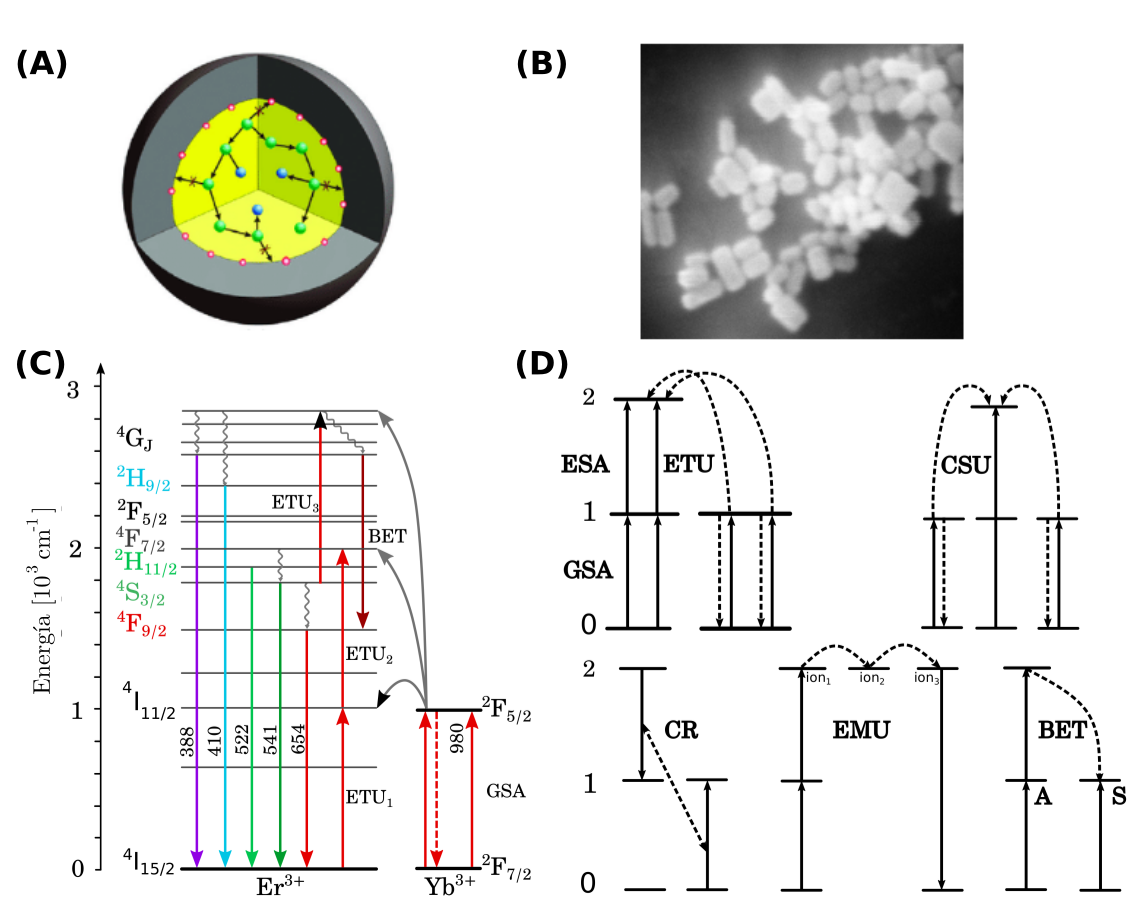
\includegraphics[width=\textwidth]{niveles_ucnp_imagen.png}
    \caption{\textbf{Diagrama de nanopartículas de \textit{upconversion}.} (\textbf{A}) Diagrama de una UCNP. Consiste en una matriz cristalina dopada con lantánidos en el interior (amarillo), y una capa externa (negro) sin dopaje. (\textbf{B}) Imagen SEM de las nanopartículas utilizadas durante esta tésis. (\textbf{C}) Diagrama de niveles de una UCNP dopada con iones de erbio Er$^{3+}$ e iterbio Yb$^{3+}$. (\textbf{D}) Mecanismos principales de interacción entre los dopantes. Tomada de \cite{bujjamer2020}.}
    \label{fig:ucnp_niveles}
\end{figure}

\subsection{Mecanismos y dinámica de las UCNP}

Para que la excitación sucesiva de los iones de erbio sea posible, distintos mecanismos de transferencia de energía se dan con el iterbio.
Un diagrama de cada uno de ellos se puede ver en la figura (\textbf{\ref{fig:ucnp_niveles}D}).
Todas las excitaciones comienzan por una excitación del nivel fundamental (\textit{Ground State Absorption}, GSA) al primero excitado en la escalera de niveles con energía de 980 nm.
Esto puede pasar tanto para el erbio como para el iterbio, pero como comentamos en la sección anterior, el iterbio tiene una sección eficaz mucho mayor, y por lo tanto es más probable que absorba un ion.
Una vez en el estado excitado, gracias a sus largos tiempos de vida, el Er tiene una probabilidad apreciable de volvera absorber otro fotón (\textit{Excited State Absorption}, ESA), excitandolo al nivel $^4$F$_{7/2}$ con energía equivalente a $\sim 490$nm.
Con menor probabilidad, la situación se podría volver a repetir.
Otra alternativa es que un ion excitado de Yb transfiera su energía de forma no radiativa a través de interacciones dipolo-dipolo a un ion de Er (\textit{Energy Transfer Upconversion}, ETU) \cite{Auzel2004}.
En este caso, el Yb vuelve a su estado fundamental sin emitir un fotón, y el Er excita su electrón de valencia a un nivel más alto.
Tanto ETU como ESA son los mecanismos más probables que causan la luminiscencia de las UCNP \cite{pollnau2000}.
\textit{Cooperative Sensitization Upconversion} (CSU) y \textit{Energy Migration Upconversion} (EMU) son mecanismos que requieren la interacción de tres iones, en los que los estados excitados se transfieren de unos a otros.
Algunos de los mecanismos, como la relajación cruzada (\textit{Cross Relaxation}, CR), no benefician la luminiscencia, sinó que la perjudican.
CR consiste en la interacción de dos electrones excitados en la que ambos quedan en un estado intermedio no radiativo.
\textit{Back Energy Transfer} (BET) es otro de este tipo, consiste en la relajación de un ion activador en un estado excitado a un sensibilizador \cite{bujjamer2020}.

Cada uno de estos mecanismos hace una contribución a la dinámica de la transición de estados de las UCNP.
A diferencia de los sistemas fluorescentes más simples como los discutidos en la sección \ref{sec:dinamica}, las ecuaciones dinámicas de las nanopartículas de \textit{upconversion} resultan en sistemas de ecuaciones más complejos.
Para empezar, hay una ecuación para cada nivel de energía excitado.
Además, cada mecanismo de transferencia agrega términos cruzados en las ecuaciones, y al depender de la presencia de fotones en más de un nivel, suelen ser términos no lineales.
Cada uno de esos términos también está acompañado por un coeficiente desconocido que describe el tiempo característico del mecanismo.
El resultado es un sistema de doce ecuaciones diferenciales ordinarias no lineales, con decenas de parámetros desconocidos \cite{anderson_revisiting_2014}.
Los términos no lineales de las ecuaciones dinámicas se asocian con la absorción secuencial de $n$ fotones que tiene que ocurrir para que las UCNP emitan luz.
Esto tiene una consecuencia directa en las observaciones de los experimentos: la luminiscencia depende de la densidad de potencia de excitación como una ley de potencias \cite{pollnau2000}.
Cada mecanismo sigue una ley de potencias con distinto exponente, pero tienen en común que están relacionadas con el número de fotones presente en el proceso.

\subsection{Requisitos para la caracterización óptica de las UCNP}

Las UCNP son un sistema luminiscente que convierte fotones de 980 nm en el NIR al espectro visible a través de múltiples interacciones entre los iones lantánidos que las componen.
Esta interacción se modela a través de un sistema de doce ecuaciones diferenciales no lineales con decenas de parámetros desconocidos.
La no linealidad del sistema implica que tanto los espectros como los tiempos de vida dependen de la densidad de potencia de excitación de forma no trivial.
Una caracterización óptica ideal de las nanopartículas requeriría ajustar los parámetros de este sistema, aunque esto resulta imposible a fines prácticos por el tamaño del espacio de parámetros y los largos tiempos de adquisición de cada experimento, especialmente a bajas potencias de excitación.

Un instrumento apropiado para caracterizar ópticamente las UCNP debería ser capaz de:

\begin{enumerate}
    \item Medir espectros estacionarios al excitar una muestra de forma continua.
    \item Medir tiempos de vida para los distintos picos de emisión de las partículas.
    \item Variar la potencia, el ciclo de trabajo y el período de excitación.
\end{enumerate}

\noindent Idealmente, el instrumento debería ser capaz de realizar mediciones de forma automática para paliar con los largos tiempos que requieren los experimentos.
En esta tésis tomamos un espectrofluorímetro antiguo Horiba PTI Quanta Master 400, lo renovamos y ampliamos sus capacidades para que cumpla con estos requisitos.
Luego, utilizamos el espectrofluorímetro renovado para caracterizar un lote de nanopartículas de \textit{upconversion} de NaYF$_4$:Er$^{3+}$,Yb${3+}$.

En el capítulo 2 describimos con detalle el \textit{hardware} del instrumento original, explicamos qué partes conservamos y cómo reemplazamos las partes que descartamos.
Posteriormente hacemos una caracterización del sistema de detección de fotones, tanto de la respuesta del \textit{hardware} como la detección de picos a través del \textit{software}.
En el capítulo 3 explicamos cuál es la estructura del \textit{software} que controla el instrumento, así como los protocolos que implementa para realizar una medición estacionaria y una dinámica.
Por último, en la primera sección del capítulo 4 utilizamos el instrumento modificado para medir el espectro estático de excitación y emisión de una muestra patrón y lo comparamos con la misma medición hecha con el instrumento original.
En la segunda sección hacemos una caracterización óptica completa de un lote de las UCNP, midiendo sus espectros estáticos en función de la potencia, así como sus tiempos de vida para los picos de mayor emisión.
Finalmente, se desarrollan las conclusiones del trabajo.

